% EXST 7152 - Final Project   
% Author: Yuan, Jumao 
% Date:   April 28th, 2015

% 2012 Kaggle Competition
% https://www.kaggle.com/c/detecting-insults-in-social-commentary

\documentclass[11pt]{article}
\usepackage[margin=2.0cm]{geometry}
\usepackage{color,soul}
\usepackage{xcolor}
\usepackage{sectsty}
\usepackage{hyperref}
\usepackage [english]{babel}
\usepackage [autostyle, english = american]{csquotes}
\usepackage{fancyhdr}
\usepackage{setspace}
\usepackage{fancyvrb} % for simple solution
\usepackage{listings,color} % for colored solution
\usepackage{cite}
\usepackage{url}
\usepackage{float}
\usepackage{amsmath}
\usepackage{csquotes}
\usepackage{geometry}
\usepackage{indentfirst}
\usepackage{graphicx}
\usepackage{eso-pic}% http://ctan.org/pkg/eso-pic
\usepackage{lipsum} % http://ctan.org/pkg/lipsum
\MakeOuterQuote{"}
\sectionfont{\color{red}}
\subsectionfont{\color{blue}}
\subsubsectionfont{\color{purple}}
\title{Text Mining: Detecting Insults in Social Commentary\\
       \hfill --\small{Kaggle 2012}}
\author{Yuan, Jumao}
\date{04/28/2015}
\usepackage{Sweave}


\begin{document}
\begin{singlespacing}
\Sconcordance{concordance:Draft.tex:Draft.Rnw:%
1 60 1 1 2 7 0 1 2 25 1 1 3 39 1 1 3 2 0 1 2 1 0 2 1 5 0 1 1 5 0 1 1 6 %
0 1 2 6 0 1 3 1 0 1 2 1 0 5 1 3 0 1 2 54 1 1 3 5 1 1 3 2 1 1 3 2 1 1 3 %
2 1 1 3 2 1 1 3 2 1 1 3 4 1 1 3 21 1}

\maketitle

\fancypagestyle{plain}{%
   \fancyhead[R]{\textit{EXST 7152 - Final Project}}
   \renewcommand{\headrulewidth}{0pt}
}

\setlength\parindent{0pt} %noindent
\singlespacing

%  Midterm Project will be presented on April, 28th, 2015 (Tuesday)

% setwd('/Users/jumaoyuan/Desktop/All_Proj_7152/Kaggle_Detect_Insult//')
% getwd()

\tableofcontents
\newpage
\doublespacing  %setspace
\begin{Schunk}
\begin{Sinput}
> getwd()
\end{Sinput}
\begin{Soutput}
[1] "/Users/jumaoyuan/Desktop/All_Proj_7152/Kaggle_Detect_Insult"
\end{Soutput}
\end{Schunk}

%Python - scikits.learn

\fbox{\begin{minipage}{35em}
All documents and materials can be downloaded in my \textbf{github} repository \par
 \underline{\url{https://github.com/jyuan4/Final_Project}}.
 \end{minipage}}
%------------------------------------ (Abstract) --------------------------------%
\section{Abstract}
The problem on Kaggle (\url{https://www.kaggle.com/c/detecting-insults-in-social-commentary}) is a single-classifier problem. Our goal is to judge if a comment is a insult or not. Here, we use TF-IDF, shot for  term frequency-inverse document frequency (\url{http://en.wikipedia.org/wiki/Tf-idf}), is a numerical statistic that is intended to reflect how important a word is to a document in a collection or corpus. Here, we use this technique to convert characters (comments) into sparse matrix, which is so called term-document matrix. In order to optimize this sparse matrix, we need decrease words variables as more as we can considering computation time and prediction accuracy. In this way, we used regular expression (\url{http://en.wikipedia.org/wiki/Regular_expression}), (abbreviated regex or regexp and sometimes called a rational expression) is a sequence of characters that forms a search pattern, mainly for use in pattern matching with strings, or string matching, i.e. "find and replace"-like operations. For example, "fuck" and "fuckkkkk" or "fuckk" are the same insulting word, and we need treat them as a single variable in the sparse matrix. After the sparse matrix is done, we applied multiple classification methods, like Logistic (Glmnet in \textbf{R}) Regression, Decision Tree for binary classification problem, Naive Bayes, Support Vector Machine (SVM), K-Nearest Neighbors, and some ensemble methods, such as Radom Forest and Gradient Boosting Method (GBM). The evaluation criteria for each model is AUC score or ROC curve. By comparing AUC score and computation time, we finally got the results and the best model.

%------------------------------------ (Problem Description) --------------------------------%
\section{Introduction} %background
Predict whether a comment posted during a public discussion is considered insulting to one of the participants.\\

The challenge is to detect when a comment from a conversation would be considered insulting to another participant in the conversation. Samples could be drawn from conversation streams like news commenting sites, magazine comments, message boards, blogs, text messages, etc.\\

The idea is to create a generalizable single-class classifier which could operate in a near real-time mode, scrubbing the filth of the internet away in one pass.

%------------------------------------ (Import Data) ------------------------------------%
\section{Data Description} %import data
All data can be downloaded from \url{https://www.kaggle.com/c/detecting-insults-in-social-commentary}.\\
The data consists of a label column followed by two attribute fields. \\

This is a single-class classification problem. The label is either 0 meaning a neutralcomment, or 1 meaning an insulting comment (neutral can be considered as notbelonging to the insult class.  Your predictions must be a real number in the range [0,1] where 1 indicates 100\% confident prediction that comment is an insult.\\

The first attribute is the time at which the comment was made. It is sometimes blank, meaning an accurate timestamp is not possible. It is in the form "YYYYMMDDhhmmss" and then the Z character. It is on a 24 hour clock and corresponds to the localtime at which the comment was originally made.\\

The second attribute is the unicode-escaped text of the content, surrounded by double-quotes. The content is mostly english language comments, with some occasional formatting. 


%------------------------------------ (Evaluation-AUC) ------------------------------------%
\section{Evaluation}
Entries will be evaluated using the area under the \textbf{receiver operator curve} (AUC). AUC was first used by the American army after the attack on Pearl Harbour, to detect Japanese aircraft from radar signals.\\

Today, it is a commonly used evaluation method for binary choose problems, which involve classifying an instance as either positive or negative. Its main advantages over other evaluation methods, such as the simpler misclassification error, are:  \\

1. It's insensitive to unbalanced datasets (datasets that have more installeds than not-installeds or vice versa).

2. For other evaluation methods, a user has to choose a cut-off point above which the target variable is part of the positive class (e.g. a logistic regression model returns any real number between 0 and 1 - the modeler might decide that predictions greater than 0.5 mean a positive class prediction while a prediction of less than 0.5 mean a negative class prediction). AUC evaluates entries at all cut-off points, giving better insight into how well the classifier is able to separate the two classes. \\

\textbf{Understanding AUC}

To understand the calculation of AUC, a few basic concepts must be introduced. For a binary choice prediction, there are four possible outcomes:\\
\begin{itemize}
\item true positive - a positive instance that is correctly classified as positive;
\item false positive - a negative instance that is incorrectly classified as positive;
\item true negative - a negative instance that is correctly classified as negative;
\item false negative - a positive instance that is incorrectly classified as negative);
\end{itemize}

These possibilities can be neatly displayed in a confusion matrix:

\begin{center}
\begin{tabular}{|l|l|l|}
\hline
  & P             & N \\ \hline
P & true positive & false positive \\ \hline
N & false positive & true positive \\
\hline
\end{tabular}
\end{center}

The true positive rate, or recall, is calculated as the number of true positives divided by the total number of positives. When identifying aircraft from radar signals, it is proportion that are correctly identified.\\

The false positive rate is calculated as the number of false positives divided by the total number of negatives. When identifying aircraft from radar signals, it is the rate of false alarms.


%------------------------------------ (Preprocessing) ------------------------------------%
\section{Data Preprocessing}
\begin{Schunk}
\begin{Sinput}
> #import data set
> data1 <- read.csv("data/train.csv")
> #delete date
> data <- data1[,-c(2)]
> write.csv(data, 'data.csv')
> names(data)
\end{Sinput}
\begin{Soutput}
[1] "Insult"  "Comment"
\end{Soutput}
\begin{Sinput}
> dim(data)
\end{Sinput}
\begin{Soutput}
[1] 3947    2
\end{Soutput}
\begin{Sinput}
> data[4,2]
\end{Sinput}
\begin{Soutput}
[1] "listen if you dont wanna get married to a man or a women DONT DO IT. what would it bother 
you if gay people got married stay in your lane do you let them do them. And your god is so nice 
but quick to judg if your not like him, thought you wasnt suppose to judge people."

3935 Levels: "_BeautifulFlaws okay I'm putting my throw back shirt &amp; cow girl boots on
seriously I'm coming ." ...
\end{Soutput}
\begin{Sinput}
> #check missing data
> length(which(data$Insult==0))+length(which(data$Insult==1))-nrow(data)
\end{Sinput}
\begin{Soutput}
[1] 0
\end{Soutput}
\begin{Sinput}
> #split data sets
> smp_size <- floor(0.70 * nrow(data))
> ## set the seed to make your partition reproductible
> set.seed(123) #fix training and testing sampling
> train_ind <- sample(seq_len(nrow(data)), size = smp_size)
> training <- data[train_ind, ]
> testing <- data[-train_ind, ]
> com.train <- training$Comment
> com.test <- testing$Comment
\end{Sinput}
\end{Schunk}
 
%------------------------------------%
\subsection{Missing values and typos}
There are two useful variables and 3947 observations in datasets. The response variable is binary, "Is Insult" or "Is Not Insult". \\

There is no missing value in the datasets, but we need do token and regular expression analysis.

%------------------------------------% 
\subsection{TF-IDF}
\begin{center}
\begin{tabular}{|p{12cm}|p{2cm}|}
\hline
\textbf{Comments}             &  \textbf{Insult} \\ \hline
"Either you are fake or extremely stupid...maybe both..."  & yes \\ \hline
"$@$tonnyb  Or they just don't pay attention"  & no \\ \hline
%\begin{verbatim}
"You with the 'racist' screen name$\backslash\backslash$n$\backslash$nYou are a PieceOfShit......"  & yes \\ \hline
"your such a dickhead..." & yes \\ \hline
\url{http://www.youtube.com/watch?v=tLYLLPHKRU4} & no \\ \hline
"You are a liar." & no \\
\hline
\end{tabular}
\end{center}

TF-IDF is used to calculate the importance of the word to each document and the weights are recorded in the new matrix. But in this case, another method in the library (library(tm) in \textbf{R}) is used to transform the sum count matrix to a tf-idf representation. Then Logistic Regression are applied on the new matrix to do the prediction.\\

There may be thousands of words included in the text, which makes the dimension of the feature set is quite high. Then it is worth figuring out if there is any way to reduce complexity of the problem. In the following two sections the author will aim at how to reduce dimensions by removing or merging some features.

\subsection{Stemming}
Another way to reduce the dimensions is to stem the words. In English, many words derive from the same stem. for instance , the words "use", "uses" "used", "useful", "using" have the same stem "use". Replacing the words with stem will reduce the size of the words in the feature set, and such a process to reduce the words to their stem is called "Stemming". There is a library called "stemDocument" in \textbf{R} providing interfaces to solve this problem. The author uses api from nltk.stem to finish the stemming process and reforms the sum count matrix, then build logistic regression on the new data set. It should be noted that PCA and Stemming can be used at the same time, so there are two models created in this section.

\subsection{Text Parsing}
Like the comment \underline{"You with the 'racist' screen name$\backslash\backslash$n$\backslash$nYou are a PieceOfShit 012......"}, we need convert upper case to lowercase, delete $\backslash$n, delete numbers (use regular expression \textbf{gsub("[$\wedge$a-zA-Z])"} in \textbf{R}) and adjust space, etc. Pieces of R codes are shown as follows:

\begin{verbatim}
dd <- Corpus(VectorSource(docs))
dd <- tm_map(dd, stripWhitespace) % Eliminating Extra White Spaces
dd <- tm_map(dd, tolower) % Convert to Lower Case
dd <- tm_map(dd, removePunctuation) % Remove Punctuations
dd <- tm_map(dd, removeWords, stopwords("english")) % Remove stopwords
%dd <- tm_map(dd, stemDocument) 
dd <- tm_map(dd, removeNumbers) % Remove numbers
dd <- tm_map(dd, stemDocument,language = 'english') % Do Stemming
\end{verbatim}

\subsection{TermDocumentMatrix}
A document-term matrix or term-document matrix is a mathematical matrix that describes the frequency of terms that occur in a collection of documents. In a document-term matrix, rows correspond to documents in the collection and columns correspond to terms. There are various schemes for determining the value that each entry in the matrix should take. One such scheme is tf-idf. They are useful in the field of natural language processing[5].

For example, for these two sentences,
\begin{itemize}
\item D1 = "I like databases"
\item D2 = "I hate databases",
\end{itemize}

\begin{center}
\begin{tabular}{|p{2cm}|p{2cm}|p{2cm}|p{2cm}|p{2cm}|}
\hline         
      & I   & like & hate & databases\\ \hline
D1 & 1 & 1      & 0      & 1 \\ \hline
D2 & 1 & 0      & 1      & 1 \\ 
\hline
\end{tabular}
\end{center}

In \textbf{R}, an object of class TermDocumentMatrix or class DocumentTermMatrix (both inheriting from a simple triplet matrix in package slam) containing a sparse term-document matrix or document-term matrix. The attribute Weighting contains the weighting applied to the matrix.

We use "TermDocumentMatrix" in \textbf{R} to constructs or coerces to a term-document matrix or a document-term matrix. The matrix is a parse matrix and will be used for later binary classification analysis with response variable "Insult".

\subsection{Feature Extraction}
The sparse matrix is huge with high dimensional variables. Lots of words will be generated in the "TermDocumentMatrix". Our main task is to downsize the high dimensional sparse matrix since the stack pointer of memory in \textbf{R} is limited (500000).

%------------------------------------%
\subsection{Split into training and testing datasets}
We randomly split data into 70\% test datasets and 30\% training datasets and repeate all models with a few iterations.


%------------------------------------ (Models) ------------------------------------%
\section{Build Moldes}
R code can be accessible on my github repository \url{https://github.com/jyuan4/Final_Project}.
%---------------- (1) KNN--------------------%
%\subsection{K-Nearest Neighbors}
%---------------- (2) NB --------------------%
%\subsection{Naive Bayes}
%---------------- (3) SVM--------------------%
%\subsection{Support Vector Machine}
%---------------- (4) Logistic--------------------%
%\subsection{Logistic (Glmnet)}
%---------------- (5) Tree--------------------%
\subsection{Classification Tree}
%R code
\begin{Schunk}
\begin{Sinput}
library(tree)
train.dat$Insult <- factor(train.dat$Insult)
# Start the clock!
ptm <- proc.time()
tree.fit <- tree(Insult~.,data=train.dat) #takes time
# Stop the clock
proc.time() - ptm
summary(tree.fit)
plot(tree.fit)
text(tree.fit, pretty=0)
tree.fit

set.seed(2)
testing$Insult <- as.factor(testing$Insult)
tree.pred <- predict(tree.fit, testing, type="class")
tree.table <- table(tree.pred, testing$Insult)

library(pROC)
roc.curve <- roc(as.numeric(tree.pred)-1, as.numeric(testing$Insult))
plot(roc.curve, main = "ROC: Classification Tree", col = "red")
auc.score<-auc(as.numeric(testing$Insult), as.numeric(tree.pred)-1)
auc.score
\end{Sinput}
\end{Schunk}

%PNG images
\begin{figure}
    \centering
    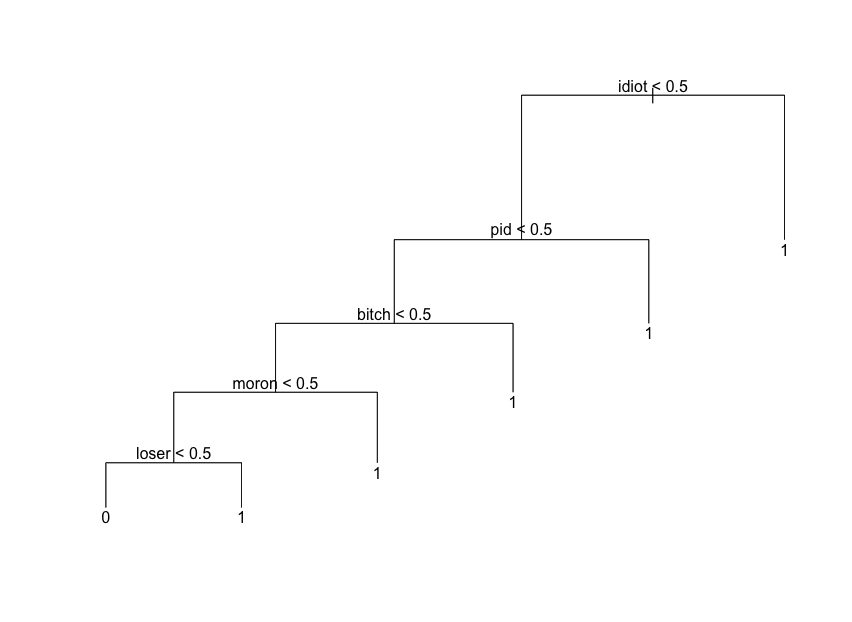
\includegraphics[width=0.8\textwidth]{tree.png}
    \caption{Classification Tree}
    \label{fig:Classification Tree}
\end{figure}



%---------------- (6) Ensemble Methods--------------------%
\subsection{Random Forest}
%R code
\begin{Schunk}
\begin{Sinput}
library(randomForest)
set.seed(100)
#500 ntree
# Start the clock!
ptm <- proc.time()
RF <- randomForest(train.dat[,1:ncol(train.dat)-1], factor(train.dat$Insult),
                   sampsize=500, do.trace=TRUE, importance=TRUE, ntree=20, forest=TRUE) #control sampsize based on rows #
# 37.454 seconds for ntree=10
# Stop the clock
proc.time() - ptm
varImpPlot(RF)
rf.pred <- data.frame(Insult.pred=predict(RF,train.dat[,1:ncol(train.dat)-1],type="prob")[,2])

library(pROC)
set.seed(10)
roc.curve <- roc(rf.pred[,1], as.numeric(train.dat$Insult))
plot(roc.curve, main = "ROC: RF", col = "red")
auc.score<-auc(as.numeric(train.dat$Insult), rf.pred[,1])
auc.score
#Area under the curve: 0.8431

rf.pred[rf.pred>=0.5] <- 1
rf.pred[rf.pred<0.5] <- 0
rf.table <- table(pred=rf.pred[,1], train.dat$Insult)
sum(diag(rf.table))/sum(rf.table) #misclassification rate
\end{Sinput}
\end{Schunk}


%PNG images
\begin{figure}
    \centering
    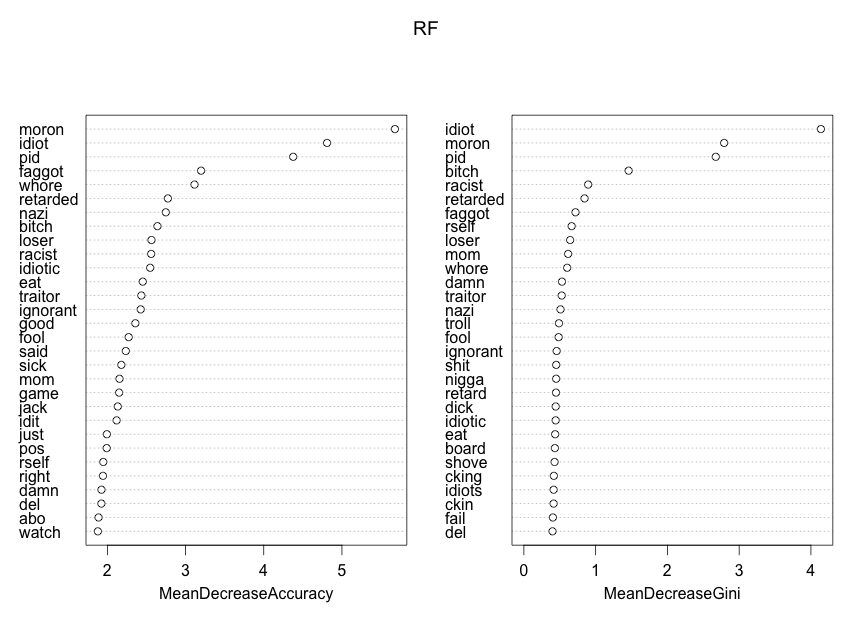
\includegraphics[width=0.8\textwidth]{rf-var.png}
    \caption{Random Forest}
    \label{fig:Random Forest}
\end{figure}

%PNG images
\begin{figure}
    \centering
    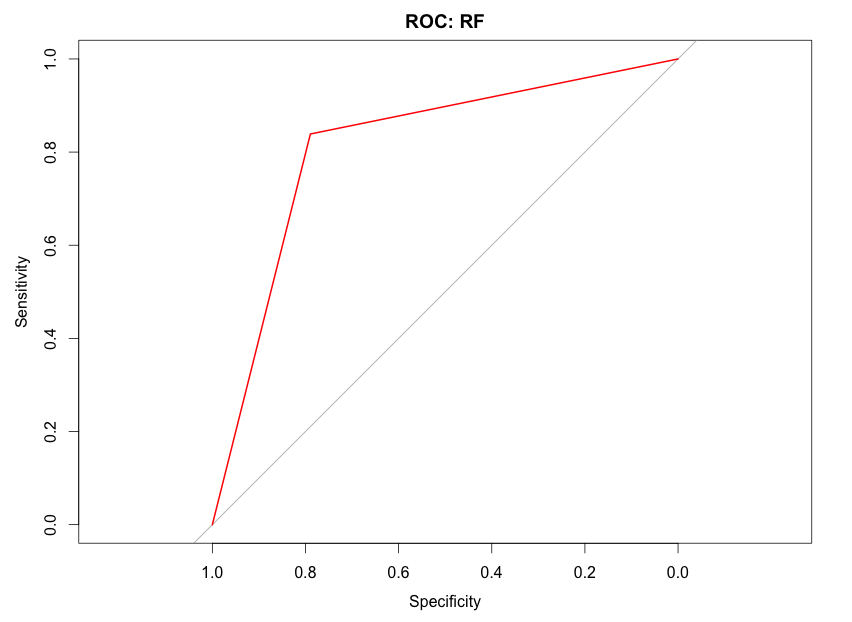
\includegraphics[width=0.8\textwidth]{rf-roc.png}
    \caption{ROC Curve}
    \label{fig:ROC Curve}
\end{figure}

%------------------------------------ (Result) ------------------------------------%
\newpage
\section{Result}
\begin{center}
\begin{tabular}{|p{4cm}|p{4cm}|p{6cm}|}
\hline         
\textbf{Method}  	& \textbf{AUC Score}   & \textbf{Computation Time (s)} \\ \hline
Random Forest 	& 0.814 		&323.362 \\ \hline
Decision Tree    	& 0.789		&46.725   \\ \hline
Logistic Regression & 0.785		& --- \\ \hline
 Naive Bayes  		& 0.798		& --- \\ \hline
KNN				& 0.730		& --- \\ \hline
SVM				& 0.786		& --- \\ 
\hline
\end{tabular}
\end{center}


%------------------------------------ (Conclusion) ------------------------------------%
\section{Conclusion and Future Work}
We have tried to investigate how to detect insults, as define in the introduction, that appear in social
discussions. To deal with it, we used some knowledge acquired during the quarter in Machine Learning.
Indeed, we started with cleaning the data, then finding relevant features and finally trying different classifiers
and designing new predictor against over-fitting. Eventually, we used our Super Predictor by combining our
predictors via AdaBoost. However, it is still difficult to detect some false negative results such as "this book
is fXXXing good" or new words (wordplays) such as "yuck fou". For these cases, we will need to find more
elaborated and complex techniques to tackle the issue.

%------------ References ------------%
\section {References}
[1]  "An Introduction to Statistical Learning" by James, G., Witten, D., Hastie, T., Tibshirani, R. \newline
[2] \url{https://www.kaggle.com/c/detecting-insults-in-social-commentary}. \newline
[3] \url{http://www.chioka.in/kaggle-competition-solutions/}. \newline
[4] \url{http://webmining.olariu.org/my-first-kaggle-competition-and-how-i-ranked/}.\newline
[5] \url{http://en.wikipedia.org/wiki/Document-term_matrix}.\newline
%[6] \url{}. \newline


%------------ End... ----------------%
\end{singlespacing}
\end{document}
